\icode{E-MV-SI-L3-260625-001}
如图所示，物块静止在水平面上，绕过光滑定滑轮的细线一端连接在物块上，另一端连接轻弹簧，轻弹簧下面吊着小球，滑轮两边的细线竖直，物块及小球均处于静止状态，将小球缓慢下拉，当物块对地面的压力恰好为零，由静止释放小球，小球做简谐运动。已知小球上升到最高点时，弹簧恰好处于原长，重力加速度大小为\(g\)，则下列说法正确的是\paren[]

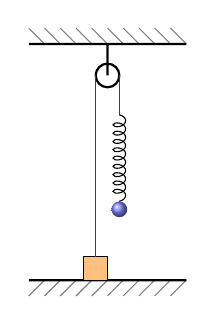
\begin{tikzpicture}
    \foreach \x in {-1,-.8,...,.8}
        {\draw[gray] (\x,-.2)--++(.2,.2);
        \draw[gray] (\x,3.2)--++(.2,-.2);}
    \draw[thick] (-1,0)--(1,0) (-1,3)--(1,3) (0,2.6) circle(.15) (0,2.6)--(0,3);
    \draw[fill=orange!50] (-.3,0) rectangle(0,.3);
    \draw[purple] (-.15,.3)--(-.15,2.6) (.15,2.6)--(.15,2.1);
    \draw[decoration={aspect=.6,segment length=3,amplitude=.8mm,coil},decorate] (.15,2.1)--(.15,1);
    \shade[ball color=blue!50] (.15,.9) circle(.1);
\end{tikzpicture}
\begin{choices}
    \item 释放小球瞬间，小球的加速度大小为\(g\)
    \item 释放小球瞬间，物块的加速度大小为\(g\)
    \item 物块的质量为小球的质量的3倍
    \item 小球向上运动过程中，重力势能和弹簧的弹性势能之和先增大后减小
\end{choices}
\begin{answer}
    A\quad 提示：小球做简谐运动，首先找到平衡位置，由释放位置到静止的位置关于平衡位置对称。
\end{answer}